%% source: 2023-sp-midterm_01
%% tags: [asymptotic notation]
\begin{prob}
    Consider the function $f(n) = n \times (\sin(n) + 1)$. A plot of this function
    is shown below:

    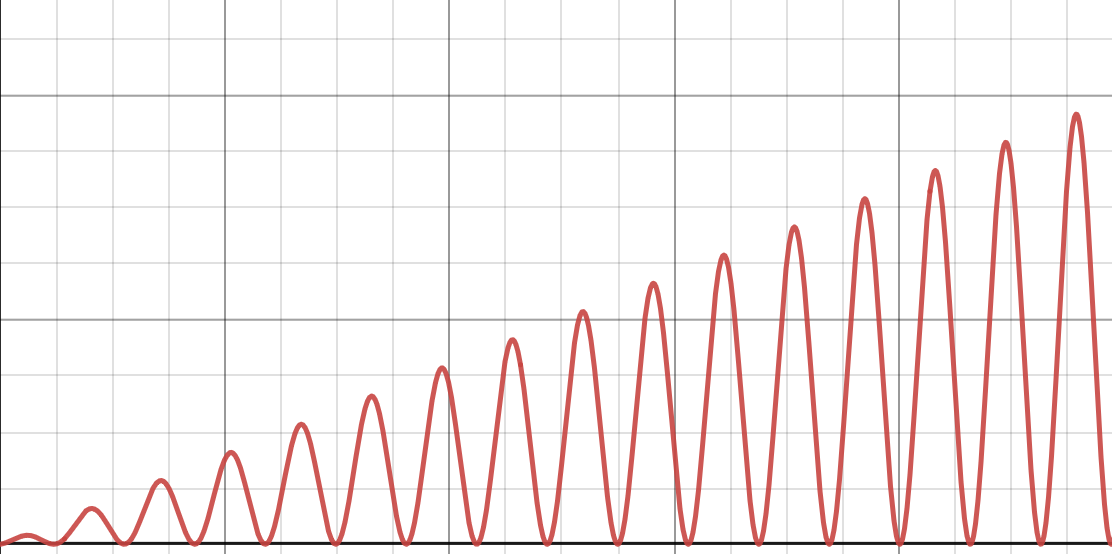
\includegraphics{./plot.png}

    True or False: this function is $O(1 + \sin n)$.

    \tF{}

    \begin{soln}
        False.

        $f(n)$ grows arbitrarily large, while $\sin n + 1$ is bounded above by 2.

        More formally, there is no constant $c$ such that $c (1 + \sin n)$
        upper bounds $f(n)$ for all large $n$.
    \end{soln}
\end{prob}
